\documentclass[12pt,a4paper]{report}
\usepackage[T1]{fontenc}
\usepackage[utf8]{inputenc}
\usepackage{charter}
\usepackage{ngerman}
\usepackage[left=2cm,right=2cm,top=2cm,bottom=2cm]{geometry}
\usepackage{graphicx}
\usepackage{amsmath}

\renewcommand\thesection{1.\arabic{section}} 

\begin{document}
	\setcounter{section}{11}
	\section{Entstehung und Eigenschaften von Wellen}
	\paragraph{(a)} Zur Entstehung von Wellen benötigen wir einen sogenannten Senderoszillator (\dq Schwingkreis als Sender\dq) und ein Medium. welches die Schwingung in den Raum trägt:\\[0.5cm]
	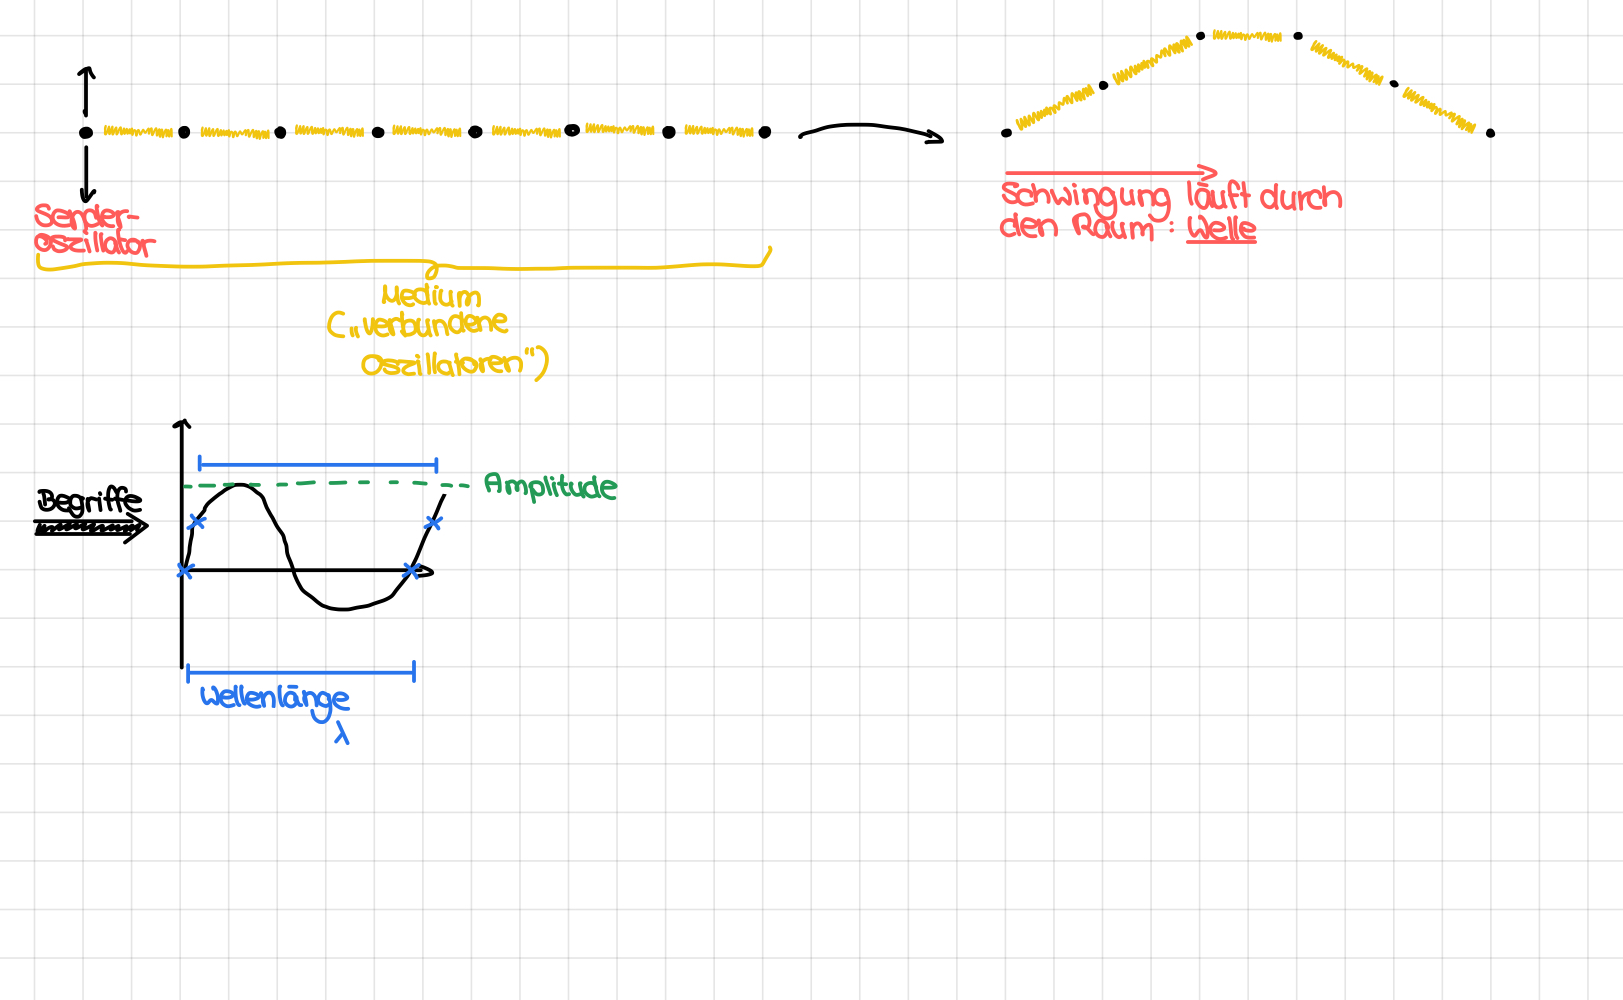
\includegraphics[width=\textwidth]{JPEG-Bild-43F1-AA6D-6C-0.JPEG}
	\\
	Die Welle kann jetzt schnell oder langsam durch das Medium laufen -- dies hängt von der Schwingung des Oszillators am Anfang ab.
	Hier ist die zeitliche Bewegung des Oszillators wichtig:
	\\[0.5cm]
	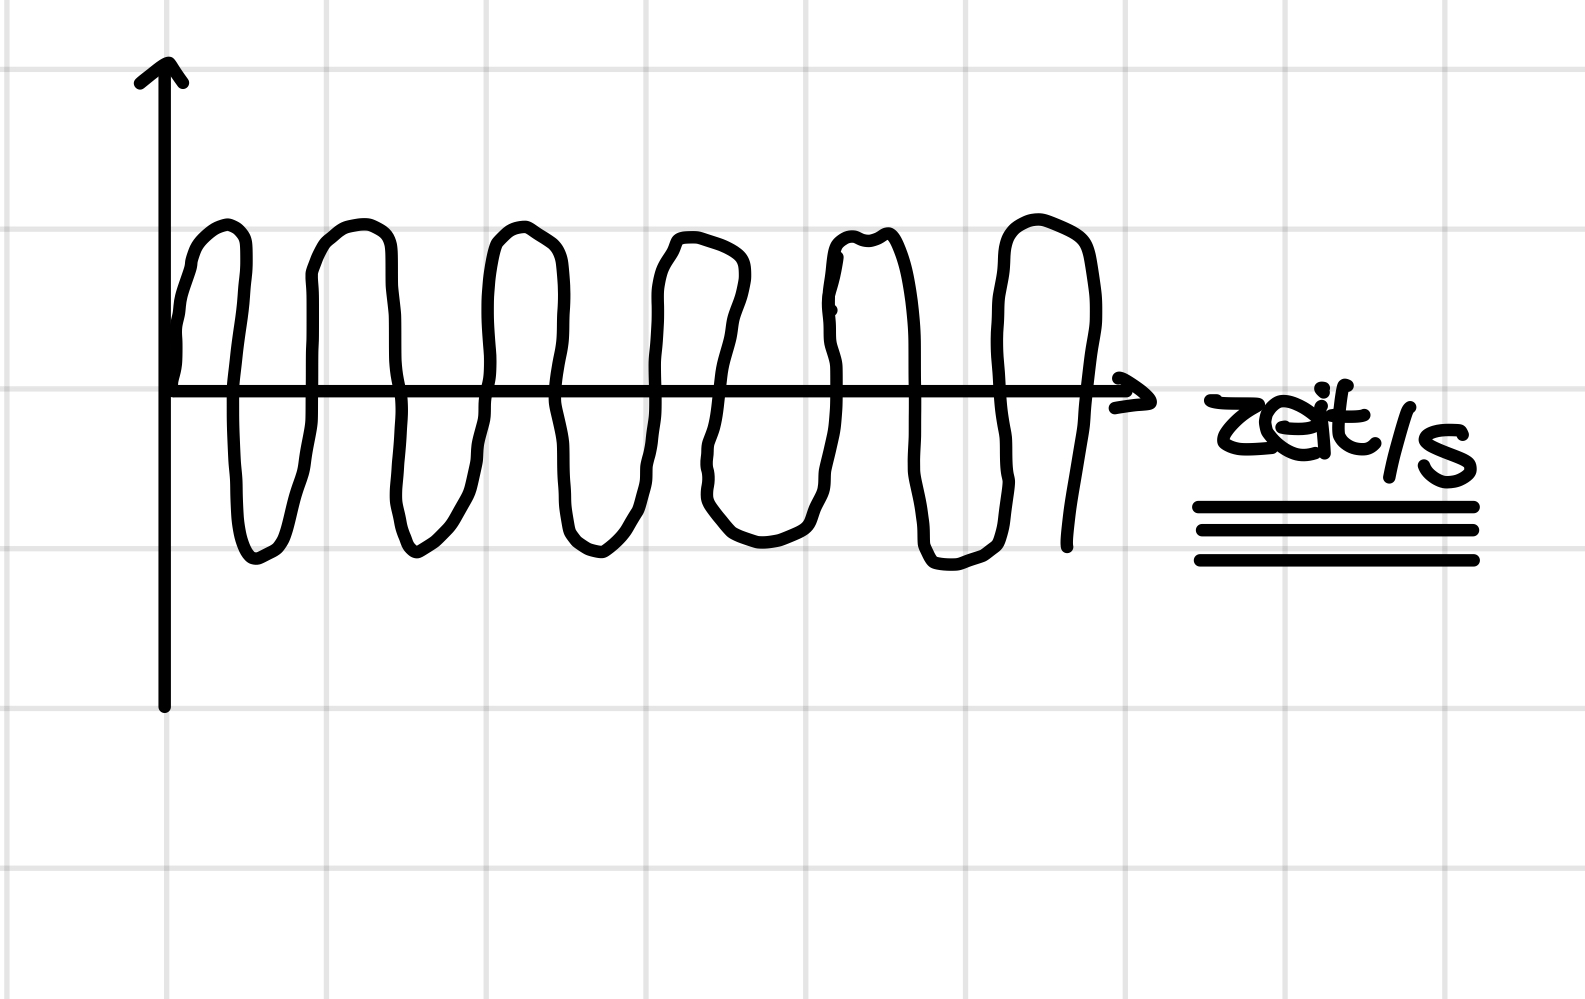
\includegraphics[width=0.5\textwidth]{JPEG-Bild-40BC-BB87-5A-0.JPEG}
	\\
	Schwingung des Oszillators mit der Frequenz f ($= \frac{1}{T}$) \\
	Geschwindigkeit der Welle:
	\begin{align*}
		C &= \frac{Weg}{Zeit} = \frac{\lambda}{T} = \lambda \cdot f
	\end{align*}
	\newpage
	\paragraph{(b)} Wellen lassen sich (nach dem Reflexionsgesetzt) reflektieren und aufhalten (absorbieren):\\[0.5cm]
	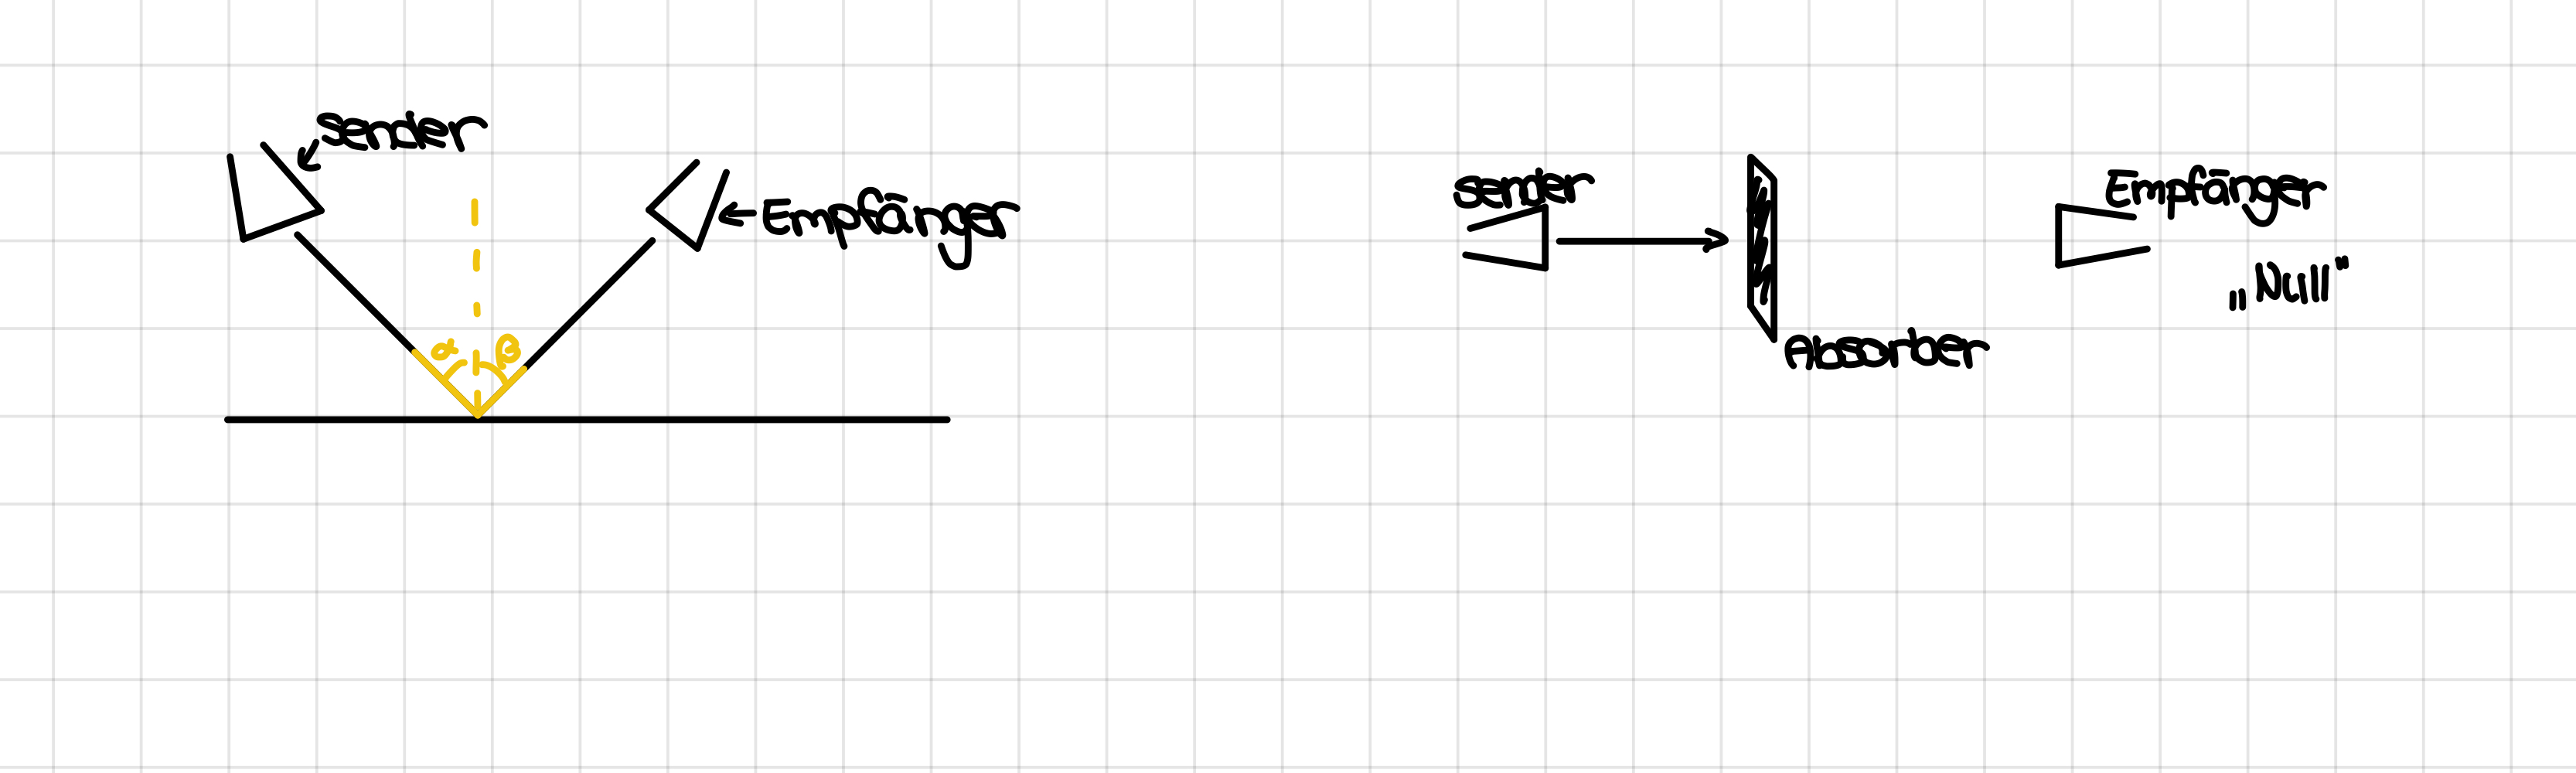
\includegraphics[width=\textwidth]{JPEG-Bild-43D0-B0E1-0A-0.JPEG}
	\paragraph{(c)} Wellen besitzen sogenannte \dq Schwingungsebenen\dq, die wir mit Polarisationsebenen bezeichnen.
\end{document}